\begin{withoutheadline}
\begin{frame}
\vspace*{-13mm}
\begin{figure}
	\hspace*{-4.2mm}
    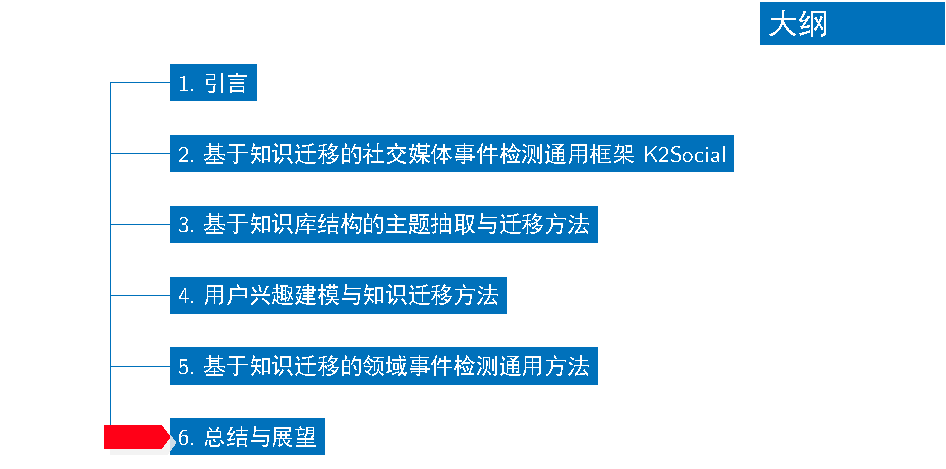
\includegraphics[width=1.0\paperwidth]{img/contents6_output.pdf}
\end{figure}

\end{frame}
\end{withoutheadline}

\section{总结与展望}
%------------------------------
\begin{frame}
\frametitle{\noindent 总结}
\begin{tikzpicture}[node distance=5mm]
\tikzset{
    every node/.style={draw, rectangle, align=center, text width=3cm, inner sep=0, thick, outer sep=0}
}
\footnotesize
\node[fill=golden, minimum height=4cm, minimum width=3cm, text width=2cm] (one) {基于知识库结构的主题抽取与迁移方法TransDetector};

\node[fill=golden, minimum height=4cm, minimum width=3cm, text width=2cm, right =of one.south east, anchor=south west] (two) {用户兴趣建模与知识迁移方法UMIETM};

\node[fill=golden, minimum height=4cm, minimum width=3cm, text width=2cm, right =of two.south east, anchor=south west] (three) {基于知识迁移的领域事件检测通用方法TransDetector$^+$};

\node[fill=red!40, fit={(one.west) (three.east)}, minimum height=1cm, above =of two] (four) {基于知识迁移的社交媒体事件检测通用框架K2Social};

\node[fill=grassgreen, text=white, fit={(one.west) (one.east)}, minimum height=1.6cm,  below= of one] (a) {提升事件检测准确性,实验中提升9\%};

\node[fill=grassgreen, text=white, fit={(one.west) (one.east)}, minimum height=1.6cm,  below= of two] (b) {提升突发事件检测时效性,实验中提前1.4小时};

\node[fill=grassgreen, text=white, fit={(one.west) (one.east)}, minimum height=1.6cm,  below= of three] (b) {提升领域事件检测准确性,实验中F值提升21\%};

\end{tikzpicture}
	
\end{frame}


%-----------------------------
\begin{frame}
\frametitle{\noindent 未来工作展望}
\begin{tikzpicture}[node distance=5mm]
\tikzset{
    every node/.style={draw, rectangle, align=center, text width=3cm, inner sep=0, thick, outer sep=0}
}
\footnotesize
\node[fill=grassgreen, text=white, minimum width=10cm, minimum height=1.6cm, text width=10cm] (a) {更多与领域相关的社会计算任务:如心理危机干预,网络亚文化社区检测等};

\node[fill=golden, minimum width=10cm, minimum height=1cm, text width=10cm, above =of a] (one) {扩展面向领域的知识迁移方法};

\node[fill=red!40, minimum width=10cm, minimum height=1cm, text width=10cm, above =of one] (four) {扩展基于知识迁移的社交媒体事件检测通用框架K2Social};

\end{tikzpicture}
	
\end{frame}